\section{The Book: An Intelligent Textbook About the Evaluation}
\label{sec:book}

The evaluation is packaged as a textbook, \textit{DGX Evaluation for Textbook Generation}, published at \url{https://dmccreary.github.io/dgx-eval/} with source at \url{https://github.com/dmccreary/dgx-eval}. The book is both the instrument's documentation and a second deliverable: it teaches a reader to repeat the evaluation on a machine of their own. This section describes what the book contains and how it was built, because the way it was built is itself an instance of the workload under test.

\subsection{Audience and Aim}

The audience is professional and continuing education: AI and machine-learning engineers, instructional technologists, technical authors, and infrastructure leads who must decide whether a local DGX can replace or supplement cloud services for generating textbooks. The assumed prerequisites are command-line comfort, basic Python and git, and experience with at least one generative AI assistant; no GPU administration, model serving, or training experience is assumed. The course description states learning outcomes at all six levels of the revised Bloom taxonomy \cite{anderson2001taxonomy}, from \textit{remember} (name the layers of the stack) to \textit{create} (a capstone that probes a machine, generates a small textbook, compares it with a cloud baseline, sanitizes every artifact, and publishes a recommendation).

The book is deliberately about \textit{decision by measurement}. It keeps three terms apart throughout: \textbf{cost}, what it takes to own and operate hardware; \textbf{price}, what a provider charges for a service; and \textbf{quality}, how good the generated textbook is. A recommendation of local, cloud, or hybrid generation has to rest on all three.

\subsection{Structure}

Table~\ref{tab:parts} summarizes the 23 chapters in six parts. The order follows the order in which a real evaluation must be done: reach the machine, verify it, choose and serve a model, connect a harness, design a fair test, and publish safely. Each setup step ends with an explicit test, so that a failure is caught at the step where it occurs and not three layers later.

\begin{table}[htbp]
\centering
\small
\begin{tabularx}{\textwidth}{@{}llX@{}}
\toprule
\textbf{Chapters} & \textbf{Part} & \textbf{What the reader does} \\
\midrule
1--2 & The target & Learn what an intelligent textbook is and the rules a generated one must follow \\
3--6 & The decision & Weigh small models against cloud services, learn the DGX hardware, separate cost, price, and quality \\
7--10 & The machine & Reach the DGX over a private mesh network, build a reproducible environment, take an inventory, probe the hardware \\
11--15 & The model & Size a model to fit in memory, select and download candidates, serve one locally, tune it \\
16--18 & The harness & Follow the agent loop, install skills, connect a harness to the local model, contain it in a sandbox \\
19--23 & The evaluation & Design a fair test, score and diagnose runs, report cost per textbook, sanitize before publishing \\
\bottomrule
\end{tabularx}
\caption{The six parts of the book. Each of the 23 chapters has an end-of-chapter quiz of ten multiple-choice questions and ten annotated references.}
\label{tab:parts}
\end{table}

\begin{figure}[htbp]
\centering
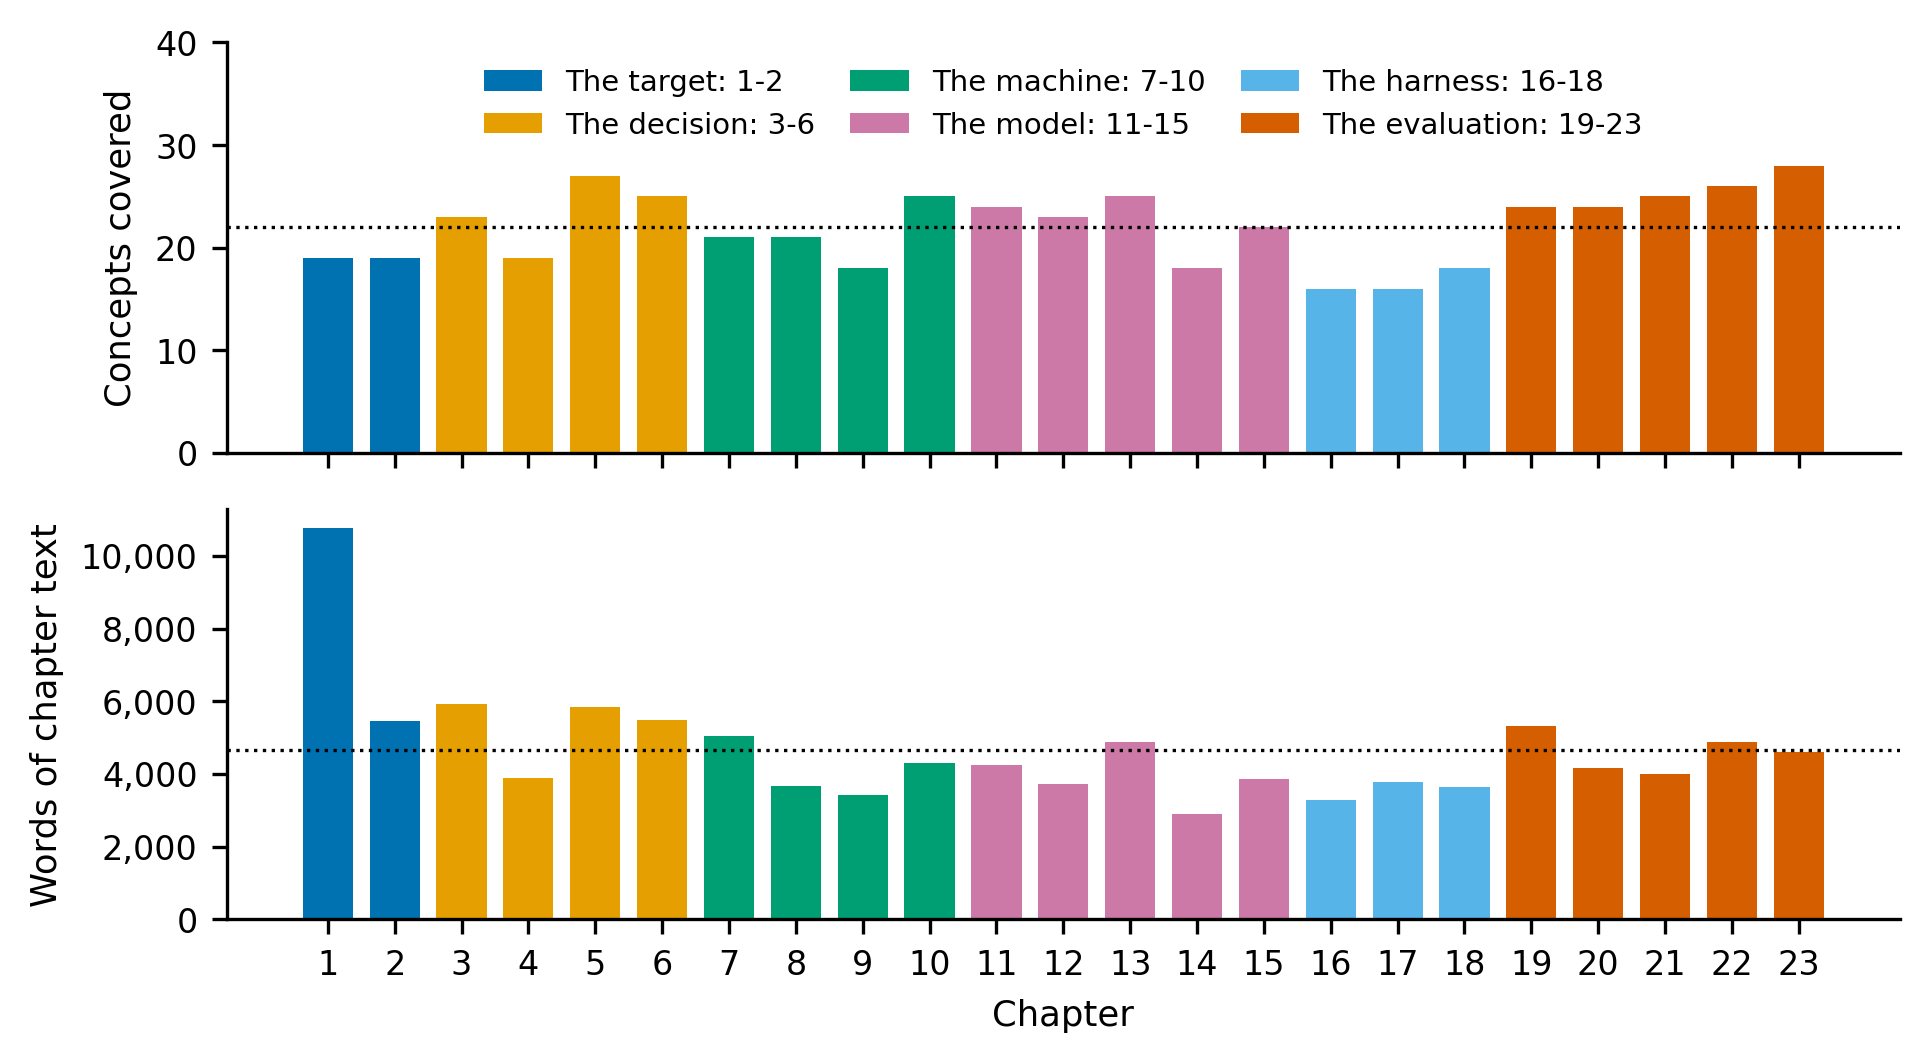
\includegraphics[width=0.95\textwidth]{figures/fig-book-structure.png}
\caption{Concepts covered and words per chapter, colored by part. Words are whitespace-delimited tokens of each chapter's source file, including tables and diagram specifications; the dotted line is the mean. Chapter~1 is long because it also carries the prerequisites, the pipeline overview, and the first worked examples.}
\label{fig:book}
\end{figure}

\subsection{Inventory}

Table~\ref{tab:inventory} counts what the book contains. The 506 concepts are not a list but a graph: 824 dependency edges, 12 foundational concepts with no prerequisite, 193 terminal concepts that nothing else depends on, no isolated node, no cycle, and a longest dependency chain of 16 concepts. Chapters were written in dependency order, so no concept is used before its prerequisites have been introduced. The longest chain runs from \textit{generative AI assistant use} through \textit{small language model} and \textit{repeated runs} to \textit{local, cloud, or hybrid decision}, which is the book's argument in miniature.

\begin{table}[htbp]
\centering
\small
\begin{tabular}{@{}lrl@{}}
\toprule
\textbf{Item} & \textbf{Count} & \textbf{Note} \\
\midrule
Chapters & 23 & about 100,000 words of chapter text \\
Concepts in the learning graph & 506 & 824 dependencies, a directed acyclic graph \\
Glossary terms & 506 & one definition per concept \\
Quiz questions & 230 & ten per chapter, tied to concepts \\
Annotated references & 230 & ten per chapter, each with a relevance note \\
MicroSims & 36 & all at status \textit{built}; none yet \textit{approved} \\
Candidate models & 10 & six with results \\
\bottomrule
\end{tabular}
\caption{What the book contains. ``Built'' means implemented and awaiting review by the author; ``approved'' is reserved for the human author after exercising the controls.}
\label{tab:inventory}
\end{table}

\subsection{Construction by the Pipeline It Evaluates}

The book was generated with the skill chain it benchmarks (Section~\ref{sec:design}): a course description was analyzed and scored, a 506-concept learning graph and taxonomy were generated, chapters were designed from the graph, chapter text was written, and then the glossary, FAQ, quizzes, and references were generated. Each chapter was sized from its own concepts. Every concept carries a Concept Impact Score (CIS): one plus the sum of the CIS of every concept that depends on it, so that a concept many others build on receives a larger word budget. This budget is the same one the conformance score of Section~\ref{sec:measurement} uses to judge generated chapters, so the book's content rules and the benchmark's scorer are one specification applied twice.

The project's agent instructions add rules a generated chapter must satisfy: anti-padding rules that prefer a dense section to a long one, a fixed layout for diagram specifications, and placement rules for the book's learning mascot. We describe them here because they are what the scorer later measures, and because the book is an unusually complete record of how a human author and an AI assistant divided the work: a design-choices page records each decision, who made it, what else was considered, and which choices did not hold up.

\subsection{Status of the Book}

The book is a working draft by an AI assistant under human direction, and it labels its generated content accordingly. The model-results pages are published exactly as each model wrote them, apart from removed links to missing pages, with a banner stating that no person has yet judged them. The MicroSims are implemented but unreviewed. Section~\ref{sec:discussion} returns to what this means for use with learners.
